\label{Chapter1}

\section{Μέρος πρώτο: εκμάθηση μιας νέας σημειακής λειτουργίας}

\subsection{Υλοποίηση της σύναρτησης solarize}

To \textbf{solarize} είναι ένας αλγόριθμος στην επεξεργασία είκονας η οποία δημιουργεί το \textbf{φαινόμενο Sabattier}.
Το φαινόμενο Sabattier είναι το φαινόμενο στις φωτογραφίες, όπου η εικόνα είναι μαγνητοσκοπημένη σε ένα αρνητικό.

\begin{problem}
	Θα πρέπει να δημιουργηθεί μία συνάρτηση, η οποία θα υλοποιεί το φαινόμενο Sabattier και στην συνέχεια θα την κάνει ασπρόμαυρη.
\end{problem}

Αυτό μπορεί να υλοποιηθεί πολύ εύκολα με την χρήση του NumPy.
Το NumPy κοιτάει τις τιμές της εικόνας και όπου είναι μεγαλύτερο από την τιμή κατωφλίου (threshold), τότε βάζει την αντίθετη τιμή, διαφορετικά δεν την αλλάζει.

\begin{lstlisting}[language=Python, caption=Solarize Function]
def solarize(image, threshold):
    return np.where((image < threshold), image, ~image)
\end{lstlisting}

\subsection{Εφαρμογή της συνάρτησης Solarize}


Η συνάρτηση θα χρησιμοποιήσει την είκονα του σχήματος~\ref{fig:zelda}. Οι τιμές του threshold πρόκειται να είναι 64, 128 και 192.

\begin{figure}[H]
	\centering
	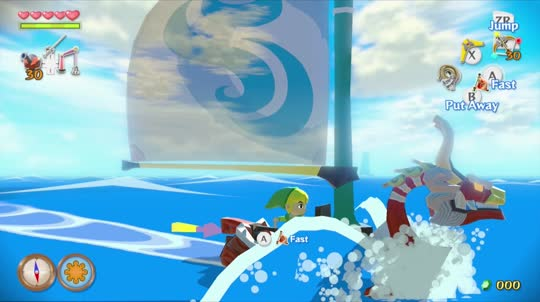
\includegraphics[width=100mm]{Figures/zelda}
	\caption[The Legend of Zelda - The Windwaker HD]{Screenshot από το βιντεοπαιχνίδι <<The Legend of Zelda - The Windwaker HD>> της Nintendo, 2013}
	\label{fig:zelda}
\end{figure}

\subsection{Αποτελέσματα εφαρμόγης}

Τα αποτελέσματα των διαφορετικών τιμών του threshold εμφανίζονται στον πίνακα~\ref{tab:threshold}.
Παρατηρώντας τα αποτελέσματα, μπορεί να παρατηρηθεί ότι όσο πιο πολύ μεγαλώνει η τιμή του threshold, τόσο πιο πολύ η original εικόνα δεν είναι αναγνωρίσιμη.

\begin{table}[H]
  \centering
	\begin{tabular}{ | p{4cm} | p{12cm} | }
		\hline
		\textbf{Τιμή threshold} & \textbf{Αποτέλεσμα} \\
		\hline
		64 & 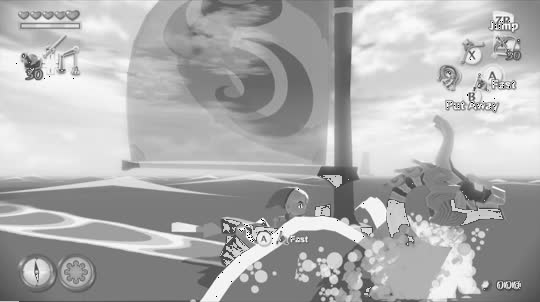
\includegraphics[width=\linewidth]{Figures/threshold_64} \\
		\hline
		128 & 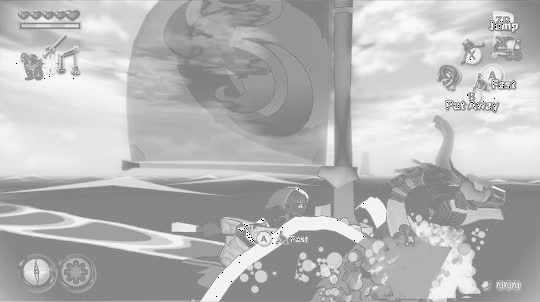
\includegraphics[width=\linewidth]{Figures/threshold_128} \\
		\hline
		192 & 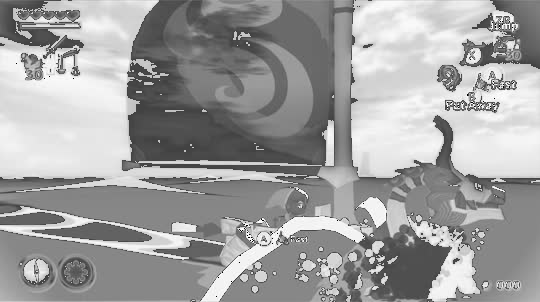
\includegraphics[width=\linewidth]{Figures/threshold_192} \\
		\hline
	\end{tabular}
  \caption{Τα αποτελέσματα των συγκρίσεων μετάξυ του πρωτότυπου και της εξομάλυνσης του Poisson}
  \label{tab:threshold}
\end{table}
